\begin{Example}[victims]{Repeat victimization}
\citet[Table 2-8]{Fienberg:80} gives the data in
\tabref{tab:victims} (from Reiss \citeyear{Reiss:80}) on instances of
repeat victimization for households in the U.S. National Crime Survey.
In this survey respondents reported all occurrences during the
period in question.  If a given household reported $n$ such incidents,
these led to $n-1$ tallies in the table, one for each pair of successive
victimizations.%
\footnote{The observation are therefore not all operationally independent
whenever $n>2$.  More detailed analysis would incorporate households
in a mixed model; however that information is unavailable here.}
%%
% Table victims written by md2tex  1-29-1998
\begin{table}[htb]
 \caption{Repeat Victimization Data}
 \label{tab:victims}
 \begin{center}
  \begin{tabular}{|l|rrrrrrrr|}
   \hline
 & \multicolumn{8}{c|}{\bfseries\large First Victimization }\rule{0in}{2.5ex}\\
{\bfseries\large Second       } &          &       &       & Pick     & Personal &      & Household & Auto    \\
{\bfseries\large Victimization} & Rape     & Assault & Robbery & Pocket & Larceny & Burglary & Larceny & Theft   \\
   \hline
% f=        2 t=        1
Rape                   &            26 &            65 &            12 &             3 &            75 &            52 &            42 &             3 \\
Assault                &            50 &          2997 &           279 &           102 &          2628 &          1117 &          1251 &           221 \\
Robbery                &            11 &           238 &           197 &            40 &           413 &           191 &           206 &            51 \\
Pick Pocket            &             6 &            85 &            36 &            61 &           329 &           102 &           117 &            24 \\
Personal Larceny           &            82 &          2553 &           459 &           243 &         12137 &          2649 &          3757 &           678 \\
Burglary               &            39 &          1083 &           197 &           115 &          2658 &          3210 &          1962 &           301 \\
Household Larceny           &            48 &          1349 &           221 &           101 &          3689 &          1973 &          4646 &           367 \\
Auto Theft             &            11 &           216 &            47 &            38 &           687 &           301 &           391 &           269 \\
   \hline
  \end{tabular}
 \end{center}
\end{table}


\figref{fig:victims1} shows the two-way mosaic for a subset of five of these
crimes (excluding pick pocket, personal larceny and household larceny).
The \chisq{} for independence is 3720.2 with 16 df.  The association
is so strong that three levels of shading were used ($|d_{ij}| \ge 2, 4, 8$).
It is at once apparent that individuals tend to be victimized repeatedly in the same way, as shown by the large blocks of positive residuals along
the main diagonal.

\begin{figure}[htb]
  \centering
  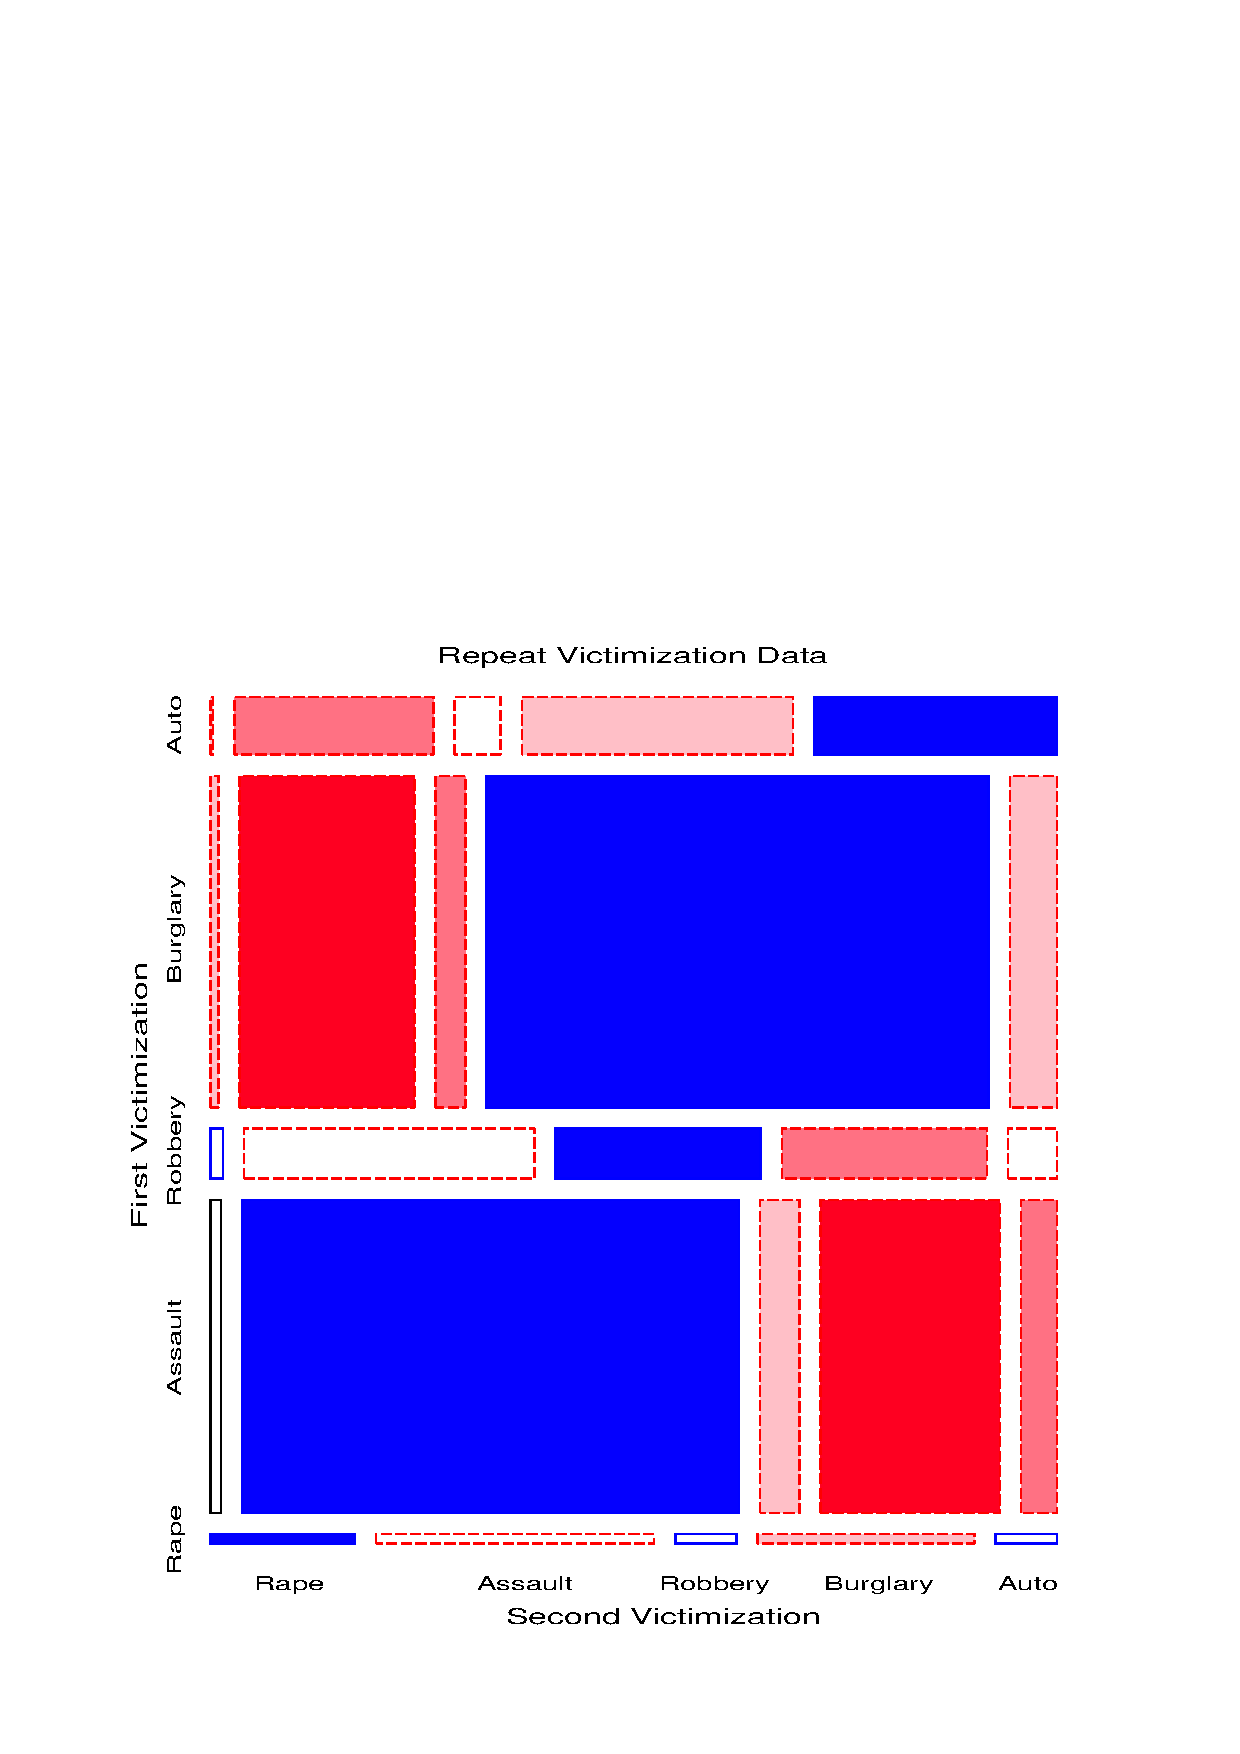
\includegraphics[scale=.6]{ch4/fig/victims1}
  \caption{Mosaic display for repeat victimization data}%
  \label{fig:victims1}
\end{figure}

\figref{fig:victims1} is produced as follows.  The statements in the
\module{victims} define the frequencies in a $8 \times 8$ matrix,
\texttt{table}.  The names of the table variables and the names of
the factor levels are defined in \texttt{vnames} and \texttt{lnames},
respectively.
%% input: /users/faculty/friendly/sasuser/mosaics/victims.sas
%% last modified: 05-May-98 15:46
\begin{listing}
goptions vsize=7 in hsize=7 in;
proc iml;
 
start victims;
   crime = \{'Rape' 'Assault' 'Robbery' 'PickPock' 'Pers.Larceny'
            'Burglary' 'Hous.Larceny' 'Auto'\};
   levels = \{8 8\};
   vnames = \{'First Victimization' 'Second Victimization'\};
   lnames = crime // crime ;
   title  = 'Repeat Victimization Data';
   table = \{  26   50  11   6    82   39   48   11,
              65 2997 238  85  2553 1083 1349  216,
              12  279 197  36   459  197  221   47,
               3  102  40  61   243  115  101   38,
              75 2628 413 329 12137 2658 3689  687,
              52 1117 191 102  2649 3210 1973  301,
              42 1251 206 117  3757 1962 4646  391,
               3  221  51  24   678  301  367  269\}`;
   finish;
   run victims;

   *-- load mosaic modules;
   reset storage=mosaic;
   load module=_all_;
 
   *-- select subset of rows/cols;
   keep = \{1 2 3 6 8\};
   table = table[keep,keep];
   lnames = lnames[,keep];
   levels = \{5 5\};

   *-- set mosaic global options;
   htext = 1.4;
   font = 'hwpsl009';
   shade = \{2 4 8\};

   plots = \{2\};
   run mosaic(levels, table, vnames, lnames, plots, title);
 
\end{listing}


There is a bit more to this story, but it is difficult to see in
\figref{fig:victims1}, owing to the large differences in the marginal
frequencies of the various crimes.  Of the crimes shown, assault and
burglary occur far more often than any others, and tend to dominate the
display.
We might therefore ask what the associations would look like if all
of these crimes occurred equally often.
As in the fourfold display, it is possible to calculate an adjusted
table (using iterative proportional fitting)
in which both sets of marginal frequencies are equally probable.

The statements below first rearrange the rows and columns of the
\texttt{table} in an order which accounts for the maximum association
and gives an opposite-corner pattern to the residuals.%
\footnote{This order is found from a correspondence analysis of
residuals, using the order of the scores on the dimension which accounts
for the largest portion of the association.}
The row totals for the crimes are used to construct an \texttt{adjusted}
table with equal marginal frequencies.
%% input: /users/faculty/friendly/sasuser/mosaics/victims.sas
%% last modified: 05-May-98 15:46
\begin{listing}
   *-- rearrange rows/cols by CA dim1;
   keep = \{2 3 1 5 4\};
   table = table[keep,keep];
   lnames = lnames[,keep];
 
   *-- standardize table to equal margins;
   avg = table[,+] / levels[1];
   newtab = repeat(avg,1,5);
   config = \{1 2\};
   call ipf(adjusted, status, levels, newtab, config, table);
   title  = 'Repeat Victimization Data, Adjusted to Equal Margins';
   lab = crime[keep];
   print title, adjusted[r=lab c=lab f=8.2];
   plots = 2;
   run mosaic(levels, adjusted, vnames, lnames, plots, title);

   *-- fit quasi-independence (ignore diagonal cells);
   title  = 'Repeat Victimization Data, Quasi Independence';
   zeros = J(5,5) - I(5);
   run mosaic(levels, adjusted, vnames, lnames, plots, title);
quit;
\end{listing}


\figref{fig:victims2} shows the mosaic for this adjusted table.
We now see that the association among the crimes is consistent
with an ordering along a dimension of crimes of violence vs. crimes
against property.  Given that someone has been a victim of one type
of crime, they are quite unlikely to be a victim of the other type
subsequently.
\begin{figure}[htb]
  \centering
  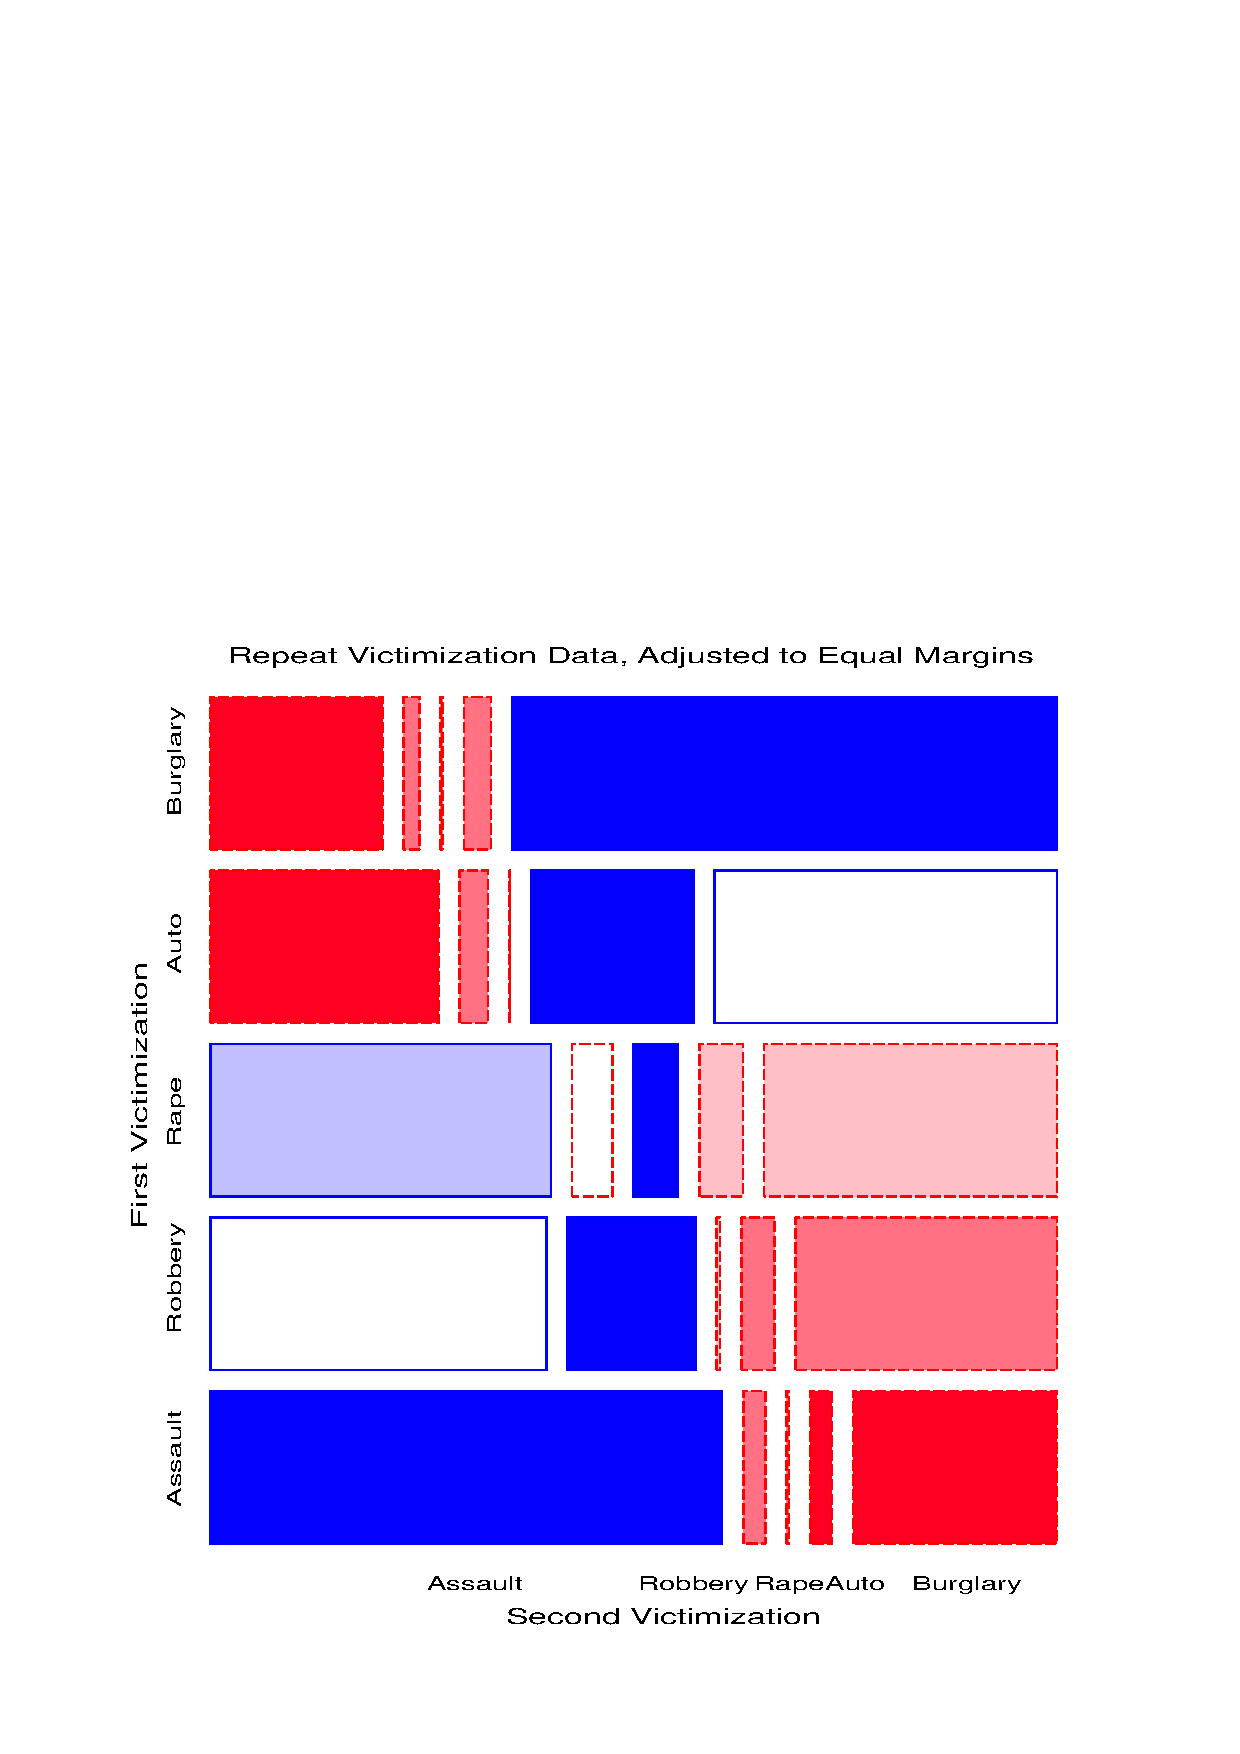
\includegraphics[scale=.6]{ch4/fig/victims2}
  \caption{Mosaic display for repeat victimization data, margins equated}%
  \label{fig:victims2}
\end{figure}

\figref{fig:victims2} is still dominated by the large positive residuals
on the diagonal representing the tendency for a person to be victimized
twice in the same way.  One way to deal with this is to fit a model
of \glossterm{quasi-independence} which ignores the diagonal cells.
This is carried out in the last call to \texttt{mosaics}.
The \texttt{zeros} matrix defines a $5 \times 5$ matrix whose values
are 0 on the diagonal and 1 elsewhere;
the value 0
indicates that the corresponding value in the \texttt{table} is to
be ignored.%
\footnote{
Zero entries cause the corresponding cell frequency to be
fitted exactly; one degree of freedom is subtracted for each
such zero.  The corresponding tile in the mosaic display is
outlined in black.}
The resulting mosaic is shown in \figref{fig:victims3}.
\begin{figure}[htb]
  \centering
  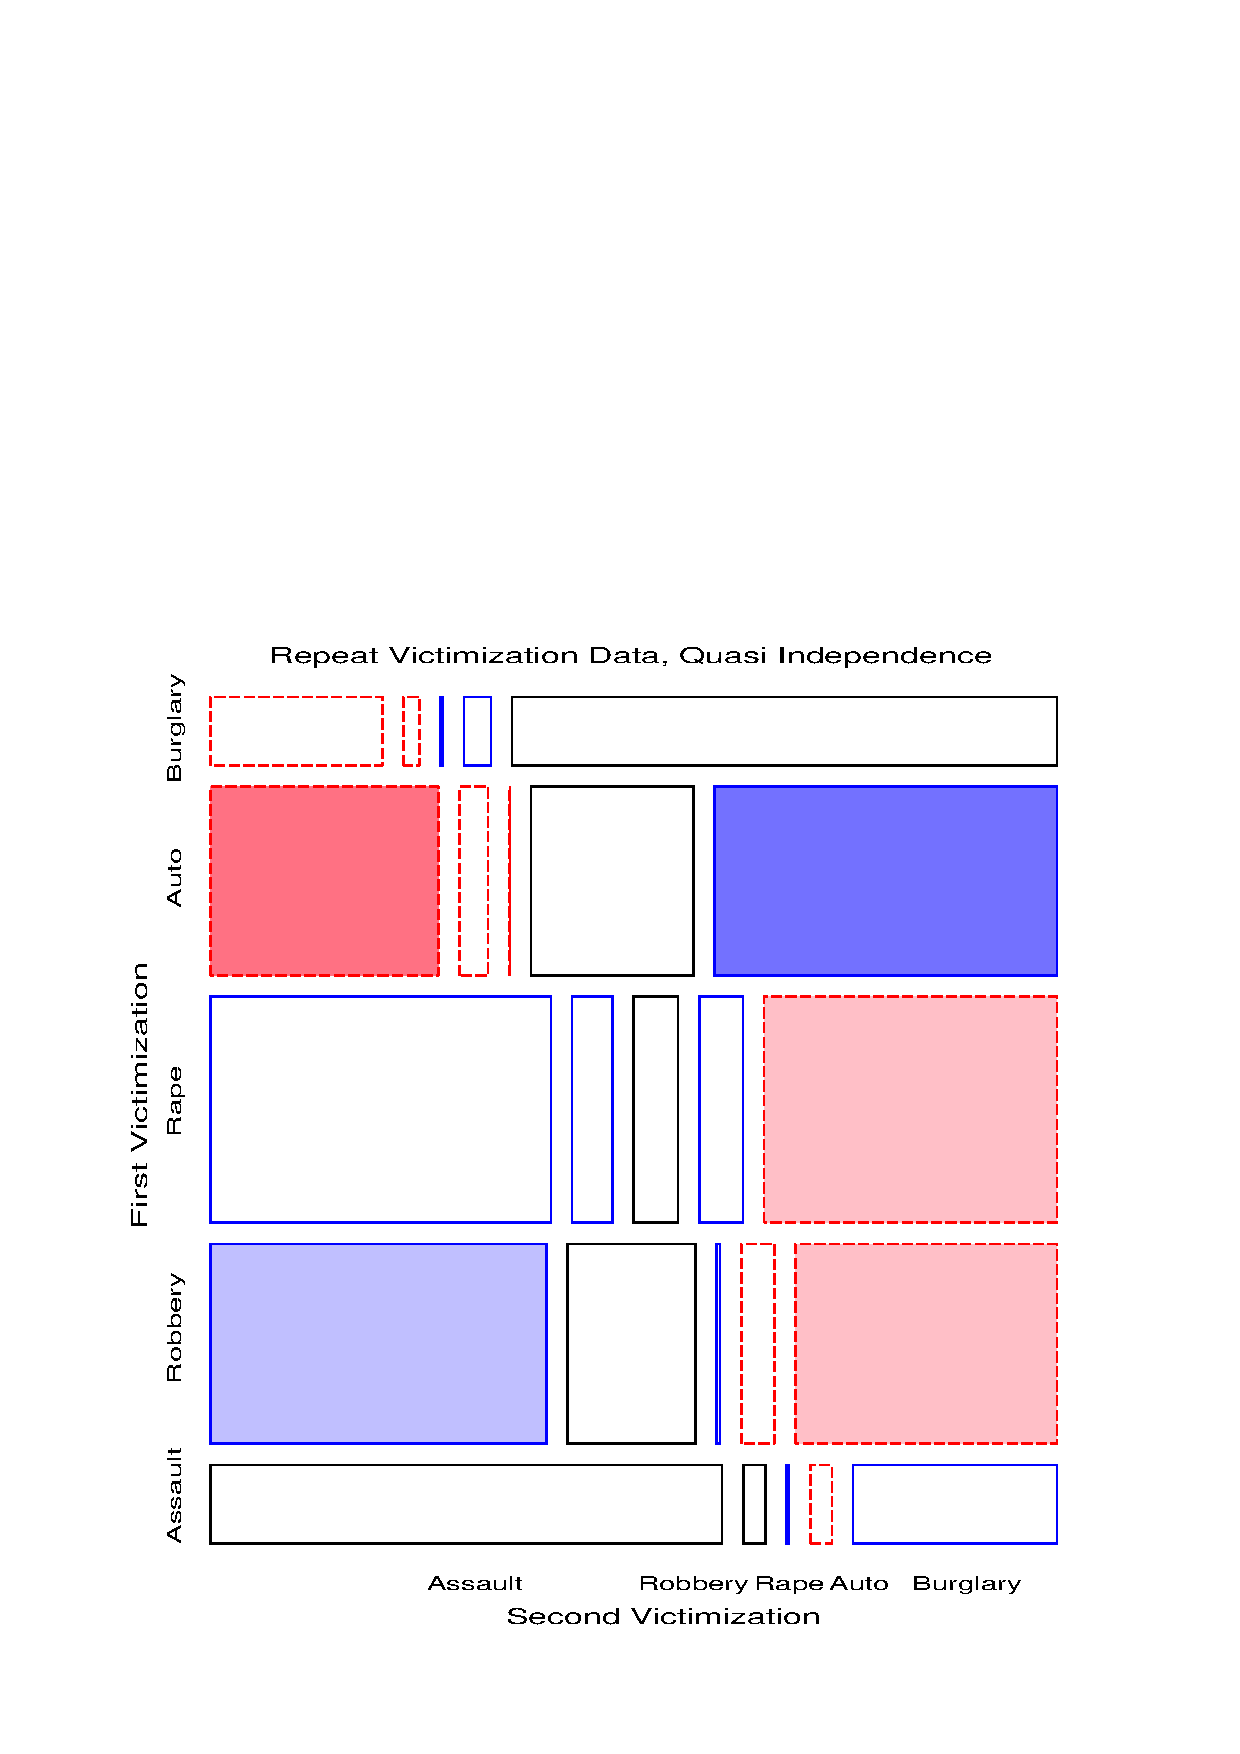
\includegraphics[scale=.6]{ch4/fig/victims3}
  \caption{Repeat victimization data, Quasi Independence}%
  \label{fig:victims3}
\end{figure}
\end{Example}
